%--------------------------------------------------------------------------------------------------
% graphic.tex
%
% This document define the section that illustrates the necessary improvements to add the
% the graphic in the simulator
%
% author: Andrea Meneghinello
% version: 0.1
%--------------------------------------------------------------------------------------------------
\section{Visualizzazione a video}
\begin{frame}{Requisiti}
	\begin{columns}
		\begin{column}{0.8\textwidth}
			Requisiti visualizzazione a video:
			\begin{itemize}
				\item{\footnotesize{ampia accessebilità alla simulazione (web browser):}}
				\begin{itemize}
					\item{\scriptsize{ampia diffusione (\tiny{pc - tablet - smartphone}\scriptsize{)}}}
					\item{\scriptsize{familiarità di utilizzo}}
					\item{\scriptsize{funzionalità HTML5 + JS}}
					\item{\scriptsize{nessun installazione richiesta}}
				\end{itemize}
				\item{\footnotesize{informazioni in tempo reale}}
				\begin{itemize}
					\item{\scriptsize{nessun polling}}
				\end{itemize}
				\item{\footnotesize{client ``leggero'':}}
				\begin{itemize}
					\item{\scriptsize{computazione lato server}}
					\item{\scriptsize{decodifica e disegno 2D}}
					\item{\scriptsize{accesso da dispositivi a ``bassa'' potenza}}
				\end{itemize}
			\end{itemize}
		\end{column}
		\begin{column}{0.2\textwidth}
			
\includegraphics[scale=0.25]{images/requirement.png}
		\end{column}
	\end{columns}
\end{frame}

\subsection{Panoramica interventi}
\begin{frame}{Panoramica interventi}
	\only<1>
	{
		\centering
		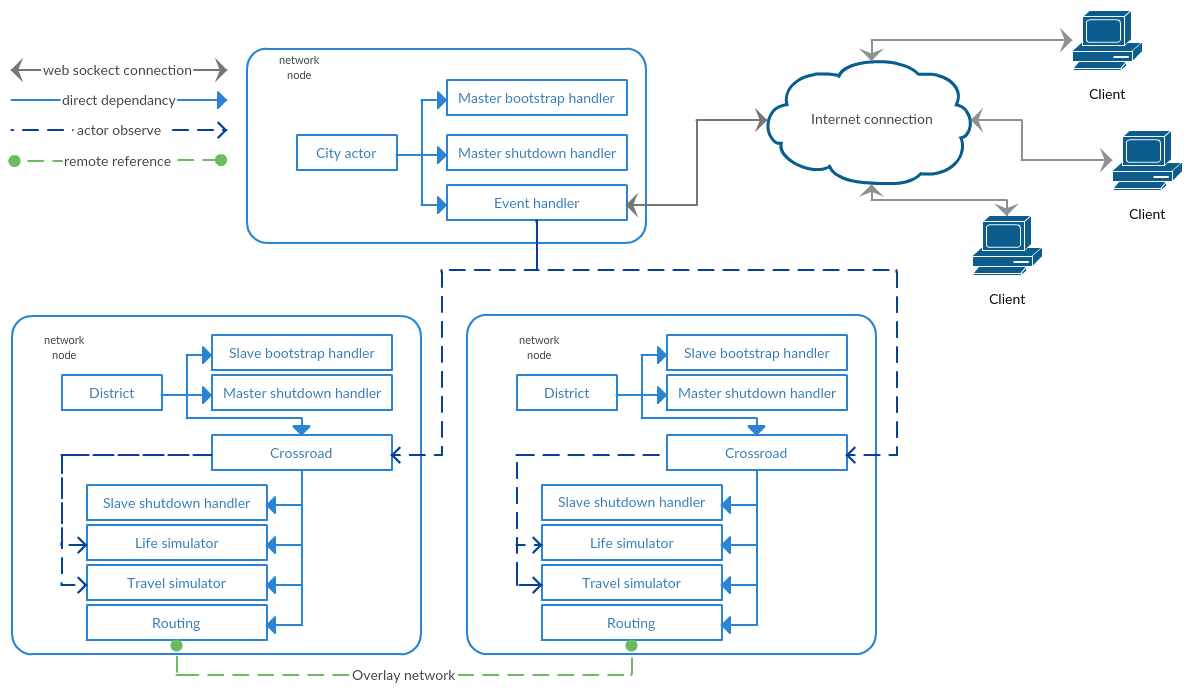
\includegraphics[scale=0.27]{images/finalDesign.png}
	}
	\only<2>
	{
		\centering
		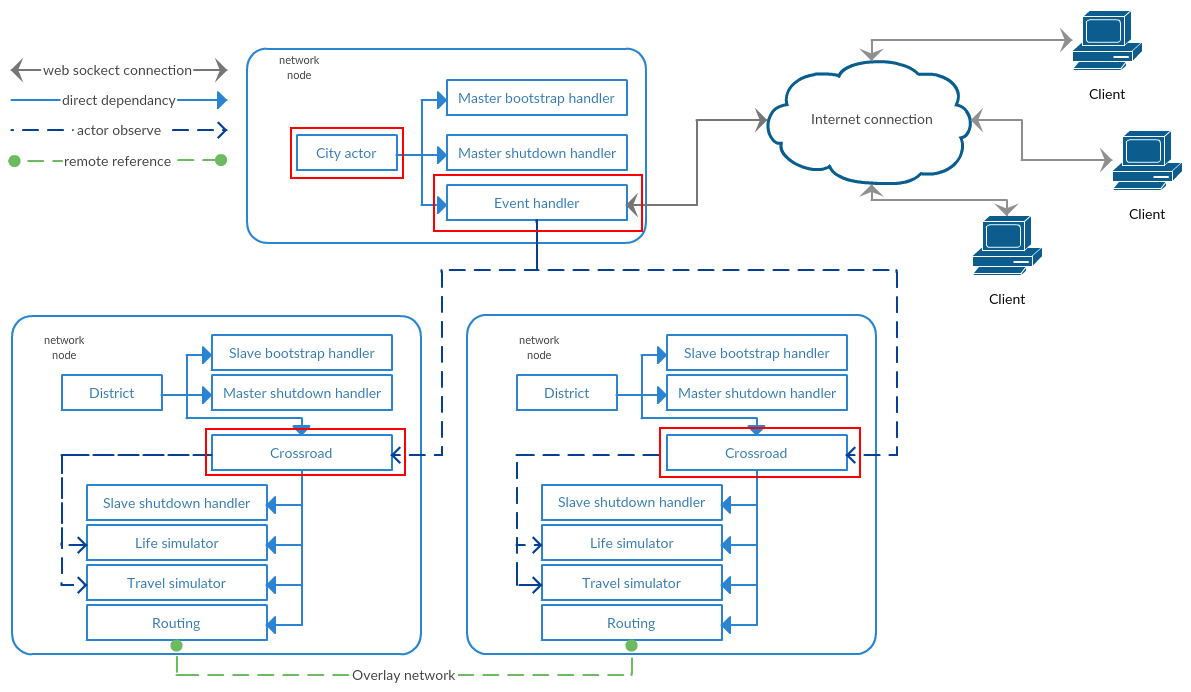
\includegraphics[scale=0.27]{images/graphicIntervents.png}
	}
\end{frame}

\subsection{Interventi nodo distretto}
\begin{frame}{Interventi nodo distretto -- \scriptsize{Crossroad}}
	\begin{columns}
		\begin{column}{0.7	\textwidth}
			Interventi:
			\begin{itemize}
				\item{\footnotesize{comportamento:}}
				\begin{itemize}
					\item{\scriptsize{forwarding dei messaggi evento}}
					\begin{itemize}
						\item{\tiny{change}}
						\item{\tiny{cross}}
						\item{\tiny{progress}}
						\item{\tiny{overtaking}}
					\end{itemize}
				\end{itemize}
				\item{\footnotesize{mailbox:}}
				\begin{itemize}
					\item{\scriptsize{definizione ``receive method'' per gestione eventi}}
					\item{\scriptsize{posto in ``or'' con l'``operation phase method''}}
				\end{itemize}
			\end{itemize}
			Risultato:
			\begin{itemize}
				\item{\footnotesize{controllo locale del ``territorio''}}
			\end{itemize}
		\end{column}		
		\begin{column}{0.3\textwidth}
			\centering
			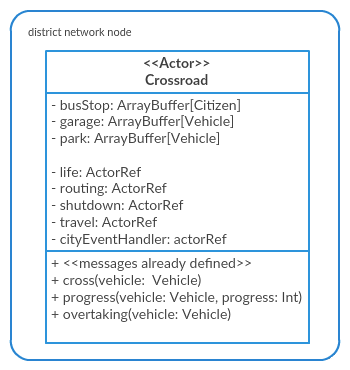
\includegraphics[scale=0.3]{images/crossroad.png}
		\end{column}
	\end{columns}
\end{frame}

\subsection{Interventi nodo città}
\begin{frame}{Interventi nodo città -- \scriptsize{gerarchia}}
	\begin{columns}
		\begin{column}{0.6\textwidth}
			Interventi:
			\begin{itemize}
				\item{\footnotesize{gestione canale di comunicazione}}
				\begin{itemize}
					\item{\scriptsize{apertura - chiusura - recupero da fallimento}}
				\end{itemize}
				\item{\footnotesize{gestione dati}}
				\begin{itemize}
					\item{\scriptsize{computazione prima della spedizione -> client leggero}}
					\item{\scriptsize{diversi output -> gerarchia attori}}
					\item{\scriptsize{modello public-subscriber}}
				\end{itemize}
			\end{itemize}
		\end{column}
		\begin{column}{0.4\textwidth}
			\centering
			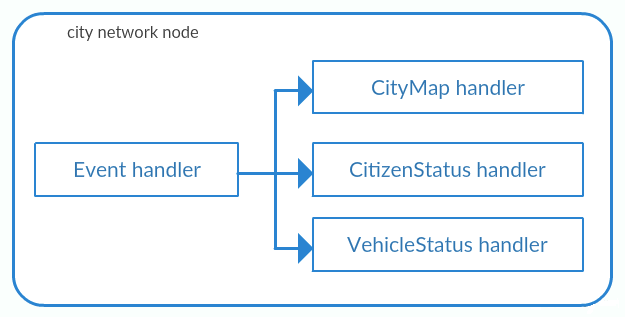
\includegraphics[scale=0.2]{images/cityEventHandlerHierarchy.png}
		\end{column}
	\end{columns}
\end{frame}

\subsubsection{WebSocket}
\begin{frame}{Interventi nodo città -- \scriptsize{WebSocket}}
	\only<1>
	{
		\centering
		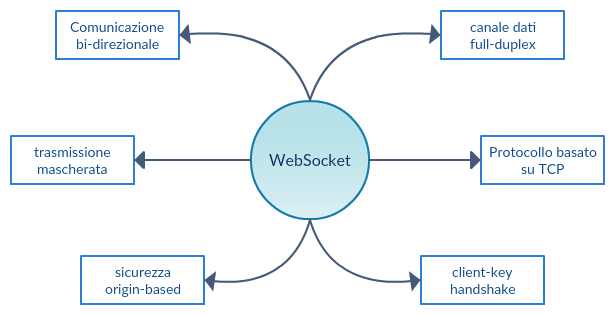
\includegraphics[scale=0.5]{images/websocketCharacteristics.png}
	}
	\only<2>
	{
		Supporto WebSocket (\scriptsize{20/01/2015}\normalsize{)}
		\centering
		\includegraphics[scale=0.25]{images/websocketSupport.png}
		\\
		\vspace{10mm}
		\tiny{fonte: canisue.com}
	}
\end{frame}

\begin{frame}{Interventi nodo città -- \scriptsize{CityEventHandler}}
	\begin{columns}
		\begin{column}{0.75\textwidth}
				Interventi:
				\begin{itemize}
					\item{\footnotesize{comportamento:}}
					\begin{itemize}
						\item{\scriptsize{connessioni + preferenze -> subclass WebSocket}}
						\item{\scriptsize{lista attori ``advertising''}}
						\item{\scriptsize{ l'invio del payload}}
					\end{itemize}
					\item{\footnotesize{mailbox:}}
					\begin{itemize}
						\item{\scriptsize{definizione ``receive method'' per gestione eventi}}
						\item{\scriptsize{posto in ``or'' con l'``operation phase method''}}
					\end{itemize}
				\end{itemize}
				Risultato:
				\begin{itemize}
					\item{\footnotesize{controllo connessioni (\tiny{recupero fallimento}\footnotesize{)}}}
					\item{\footnotesize{delega del processo di costruzione payload}}
				\end{itemize}
		\end{column}
		\begin{column}{0.25\textwidth}
			\vspace{15mm}
			\centering
			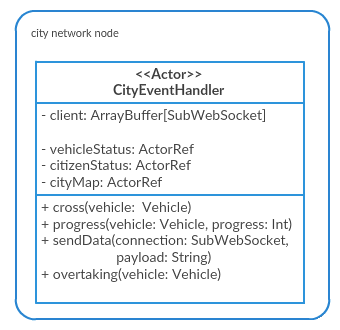
\includegraphics[scale=0.25]{images/cityEventHandler.png}
		\end{column}
	\end{columns}
\end{frame}

\begin{frame}{Interventi nodo città -- \scriptsize{CityMapHandler}}
	\begin{columns}
		\begin{column}{0.7\textwidth}
		Interventi:
		\begin{itemize}
			\item{\footnotesize{comportamento:}}
			\begin{itemize}
				\item{\scriptsize{conversione struttura cittadina}}
				\begin{itemize}
					\item{\tiny{da XML a JSON}}
					\item{\tiny{sulla base delle preferenze (risoluzione)}}
					\item{\tiny{lista incroci suddivisa per distretti}}
				\end{itemize}
			\end{itemize}
			\item{\footnotesize{mailbox}}:
			\begin{itemize}
				\item{\scriptsize{gestione nuova connessione in ingresso}}
			\end{itemize}
		\end{itemize}
		Risultato:
		\begin{itemize}
			\item{\footnotesize{gestione piantina secondo esigenze del client}}
		\end{itemize}
		\end{column}
		\begin{column}{0.3\textwidth}
			\centering
			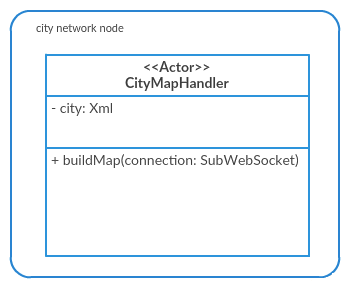
\includegraphics[scale=0.3]{images/cityMapHandler.png}
		\end{column}
	\end{columns}
\end{frame}

\begin{frame}{Interventi nodo città -- \scriptsize{CitizenStatusHandler}}
	\begin{columns}
		\begin{column}{0.6\textwidth}
			Interventi:
			\begin{itemize}
				\item{\footnotesize{comportamento:}}
				\begin{itemize}
					\item{\scriptsize{costruzione stato del cittadino}}
					\item{\scriptsize{formato JSON}}
				\end{itemize}
				\item{\footnotesize{mailbox:}}
				\begin{itemize}
					\item{\scriptsize{gestione eventi in ingresso dalle componenti del simulatore}}
				\end{itemize}
			\end{itemize}
			Risultato:
			\begin{itemize}
				\item{\footnotesize{gestione dell'output formato LOG}}
			\end{itemize}
		\end{column}
		\begin{column}{0.4\textwidth}
			\centering
			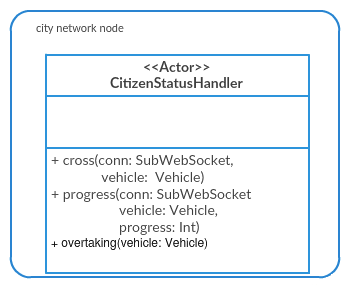
\includegraphics[scale=0.35]{images/citizenStatusHandler.png}
		\end{column}
	\end{columns}
\end{frame}

\begin{frame}{Interventi nodo città -- \scriptsize{VehicleStatusHandler}}
	\begin{columns}
		\begin{column}{0.6\textwidth}
			Interventi:
			\begin{itemize}
				\item{\footnotesize{comportamento:}}
				\begin{itemize}
					\item{\scriptsize{conversione progresso}}
					\item{\scriptsize{progresso -> coord. geogr. -> px}}
				\end{itemize}
				\item{\footnotesize{mailbox:}}
				\begin{itemize}
					\item{\scriptsize{gestione eventi in ingresso dalle componenti del simulatore}}
				\end{itemize}
			\end{itemize}
			Risultato:
			\begin{itemize}
				\item{\footnotesize{gestione output secondo esigenze specifiche}}
			\end{itemize}
		\end{column}
		\begin{column}{0.4\textwidth}
			\centering
			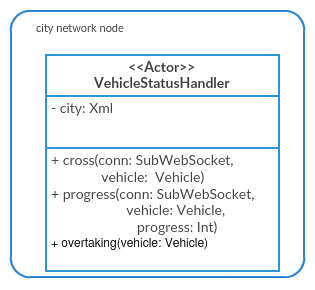
\includegraphics[scale=0.35]{images/vehicleStatusHandler.png}
		\end{column}
	\end{columns}
\end{frame}

\subsection{Algoritmo di pubblicazione}
\begin{frame}{Algoritmo di pubblicazione}
	\centering
	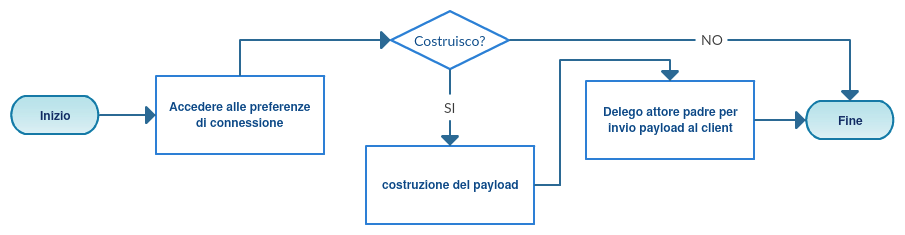
\includegraphics[scale=0.35]{images/shipPhase.png}
\end{frame}

\subsection{fasi}
\begin{frame}{Fase di connessione}
	Connessione nuovo client
	\centering
	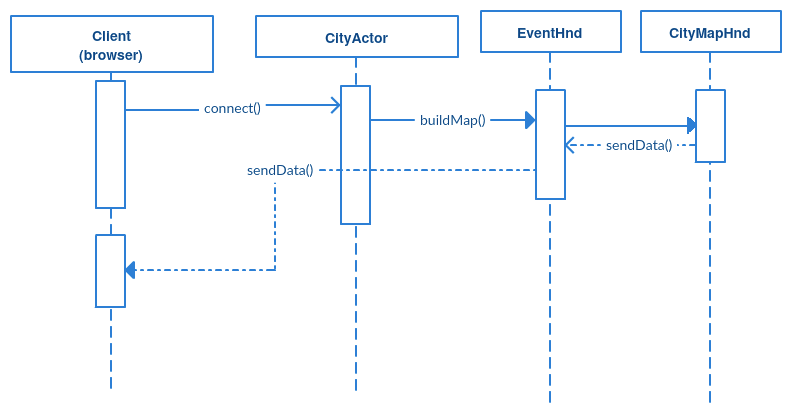
\includegraphics[scale=0.3]{images/connectionPhase.png}
\end{frame}

\begin{frame}{Ricezione di un nuovo evento}
	Propagazione di un evento
	\centering
	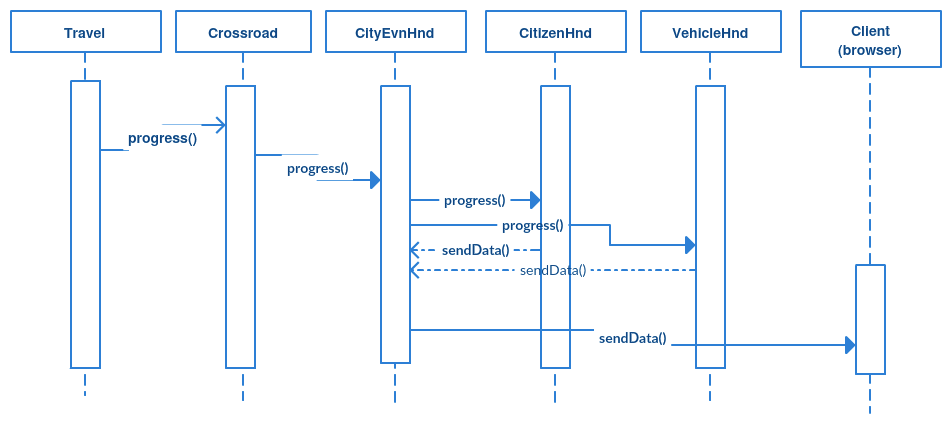
\includegraphics[scale=0.3]{images/eventTransmission.png}
\end{frame}

\subsection{Riassunto tecnologie}
\begin{frame}{Riassunto tecnologie}
	\only<1>
	{
		\begin{columns}
			\begin{column}{0.7\textwidth}
				Riassunto tecnologie:
				\begin{itemize}
					\item{\footnotesize{connessione client/server:}}
					\begin{itemize}
						\item{\scriptsize{play framework (gestione WebSocket)}}
					\end{itemize}
					\item{\footnotesize{gestione pagina web:}}
					\begin{itemize}
						\item{\scriptsize{HTML5 + CSS3 (canvas)}}
						\item{\scriptsize{bootstrap}}
						\item{\scriptsize{processing.js (gestione canvas)}}
					\end{itemize}
				\end{itemize}
			\end{column}
			\begin{column}{0.3\textwidth}
				\centering
				
\includegraphics[scale=0.15]{images/technologies.png}
			\end{column}
		\end{columns}
	}
	\only<2>
	{
		Supporto HTML5 Canvas (\scriptsize{20/01/2015}\normalsize{)}
		\centering
		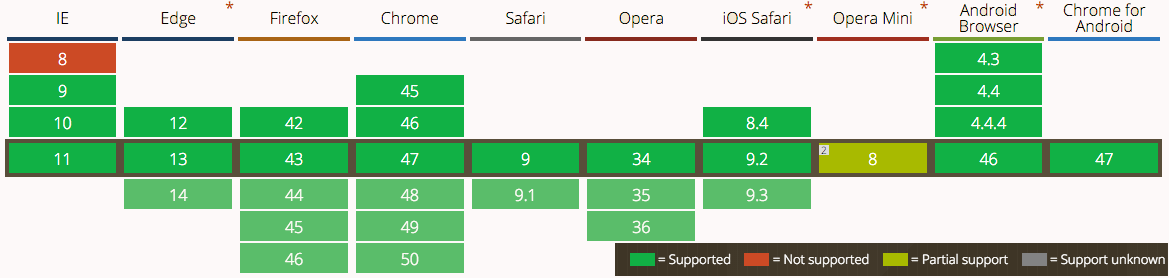
\includegraphics[scale=0.25]{images/canvasSupport.png}
		\\
		\vspace{10mm}
		\tiny{fonte: canisue.com}
	}
\end{frame}